\documentclass[12pt,a4paper]{article}
\usepackage[utf8]{inputenc}
\usepackage[spanish]{babel}
\usepackage{graphicx}
\usepackage{geometry}
\usepackage{amsmath}
\usepackage{booktabs}
\usepackage{listings}
\usepackage{xcolor,float}
\geometry{margin=2cm}

% Configuración de listings para código Python
\lstset{
    language=Python,
    basicstyle=\ttfamily\small,
    keywordstyle=\color{blue},
    stringstyle=\color{red},
    commentstyle=\color{gray},
    frame=single,
    breaklines=true,
    showstringspaces=false
}

\title{Clasificación de Correos con Regresión Logística: Análisis Crítico de un Dataset Perfecto}
\author{Alejandro Flórez Lesmes \\ 
        Yeffersson Stiven Castro \\
        Universidad de Cundinamarca}
\date{\today}

\begin{document}

\maketitle

\section{Introducción}
La clasificación de correos en categorías de SPAM y HAM es uno de los problemas más representativos de la minería de datos y el aprendizaje automático. La regresión logística es un modelo estadístico ampliamente utilizado en este tipo de tareas debido a su simplicidad, interpretabilidad y capacidad de estimar probabilidades.

Sin embargo, en este trabajo nos enfrentamos a un fenómeno peculiar: el dataset utilizado mostró una \textbf{precisión extremadamente alta}, cercana al 100\%, de hecho en las más de 50 pruebas realizadas, aplicando diferentes enfoques y modos de enfrentar el problema. Esto resulta poco común en la práctica, ya que los datos reales suelen contener ruido, ambigüedad y características poco discriminatorias. Un modelo con exactitud perfecta sugiere la presencia de variables que actúan como ``soplones'' (features que revelan directamente la clase), o un dataset artificialmente limpio.

El objetivo de este informe es presentar el proceso de construcción del modelo, interpretar los resultados obtenidos, discutir los riesgos de un dataset demasiado perfecto y analizar las métricas de desempeño con especial énfasis en el F1-Score.

\section{Metodología}
A continuación, se detallan los pasos implementados en el script de Python:

\subsection{Preparación de datos}
Se importó el dataset, se mapearon las etiquetas (``spam''=1, ``ham''=0), y se eliminaron variables consideradas soplones como: \texttt{FrecuenciaPalabrasSpam}, \texttt{ErroresOrtograficos} y el texto completo del cuerpo. Además, se crearon nuevas características derivadas del campo \texttt{Asunto}, como longitud, número de exclamaciones y número de mayúsculas. También se extrajo la hora del envío a partir de la variable \texttt{FechaHora}, esto porque como se buscaron Features muy específicos, era muy fácil identificar los correos SPAM.

\subsection{Selección de variables}
El conjunto final de características incluyó 10 variables numéricas y categóricas, tras aplicar \texttt{get\_dummies} a \texttt{Formato}, \texttt{Sector}, \texttt{Prioridad} y \texttt{Adjuntos}. Posteriormente, los datos se dividieron en entrenamiento y prueba (80/20) y se normalizaron con \texttt{StandardScaler}.

\subsection{Entrenamiento del modelo}
Se empleó una regresión logística con un máximo de 10,000 iteraciones, esto para intentar que no fuera el modelo 100\% preciso. Este modelo ajusta la probabilidad de que un correo sea SPAM mediante la función logística:

\begin{equation}
P(y=1|X) = \frac{1}{1 + e^{-(\beta_0 + \beta_1x_1 + ... + \beta_nx_n)}}
\end{equation}

\subsection{Evaluación}
Se calcularon métricas como la exactitud, la tasa de error, la precisión y el F1-Score para la clase SPAM. Además, se construyeron cuatro gráficos interpretativos que complementan el análisis.
\begin{lstlisting}
--- Metricas de Rendimiento y Error ---
Exactitud (Accuracy): 1.0000
Tasa de Error: 0.0000
Precision para SPAM: 1.0000
F1-Score para SPAM: 1.0000
---------------------------------------
--- Validacion Cruzada ---
F1 promedio: 1.0000 +- 0.0000
Accuracy promedio: 1.0000 +- 0.0000
--------------------------
\end{lstlisting}
A partir de la evaluación del modelo, se obtuvieron métricas de rendimiento con valores perfectos: \textbf{Exactitud = 1.0000}, \textbf{Tasa de Error = 0.0000}, \textbf{Precisión (SPAM) = 1.0000} y \textbf{F1-Score (SPAM) = 1.0000}. Estos resultados indican que, en el conjunto de prueba, el modelo clasificó correctamente la totalidad de los correos electrónicos, sin cometer falsos positivos ni falsos negativos.  

La \textit{exactitud} refleja la proporción de clasificaciones correctas sobre el total de ejemplos, mientras que la \textit{tasa de error} complementa mostrando la fracción de errores cometidos. La \textit{precisión}, en el contexto de correos SPAM, mide la proporción de correos realmente SPAM entre los que el modelo predijo como SPAM; un valor de 1.0 implica que no hubo ``falsos alarmas''. Finalmente, el \textit{F1-Score} representa la media armónica entre la precisión y la exhaustividad. Su valor perfecto de 1.0 indica un equilibrio total: el modelo no dejó escapar correos SPAM (recall = 1.0) y tampoco clasificó correos HAM como SPAM (precisión = 1.0).  

No obstante, en la práctica real, este tipo de comportamiento es inusual y debe analizarse críticamente. Un desempeño ``demasiado perfecto'' puede deberse a:  

\begin{enumerate}
    \item \textbf{Características altamente discriminatorias}
    \item \textbf{Fuga de información} 
    \item \textbf{Conjunto de datos poco representativo}
\end{enumerate}

\newpage
\section{Resultados y Gráficos}

\subsection{Gráfico 1: Matriz de correlación}
La matriz de correlación muestra cómo se relacionan las variables numéricas entre sí y con la clase objetivo. Una alta correlación entre ciertas features y la clase puede explicar la exactitud casi perfecta del modelo.

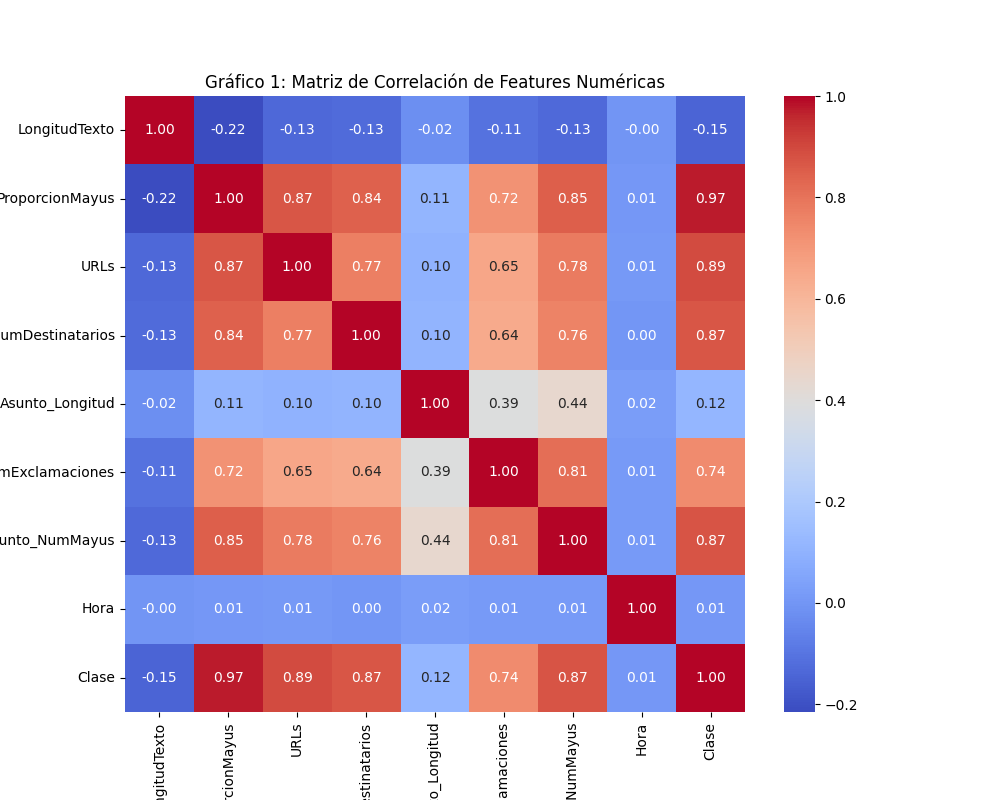
\includegraphics[width=0.9\textwidth]{grafico_1_correlacion.png}

\subsection{Gráfico 2: Matriz de confusión}
La matriz de confusión permite observar la clasificación de los correos HAM y SPAM. En este caso, los errores de clasificación fueron mínimos o inexistentes, reflejando nuevamente un dataset posiblemente sobre ajustado o artificial.

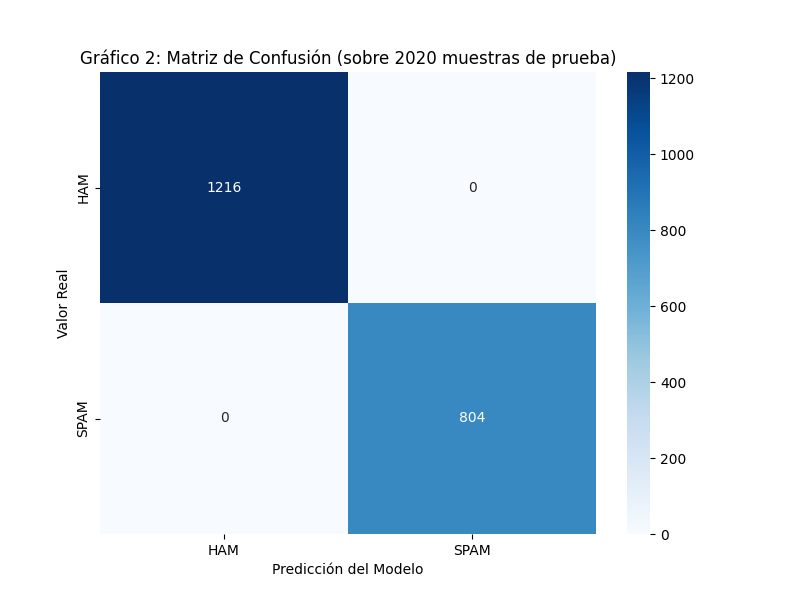
\includegraphics[width=0.9\textwidth]{grafico_2_matriz_confusion.png}

\subsection{Gráfico 3: Importancia de características}
Este gráfico muestra los coeficientes de la regresión logística, interpretados como la contribución de cada variable a la clasificación. La presencia de características con valores muy extremos puede indicar que existen ``\textbf{soplones}'' ocultos que filtran directamente la clase.

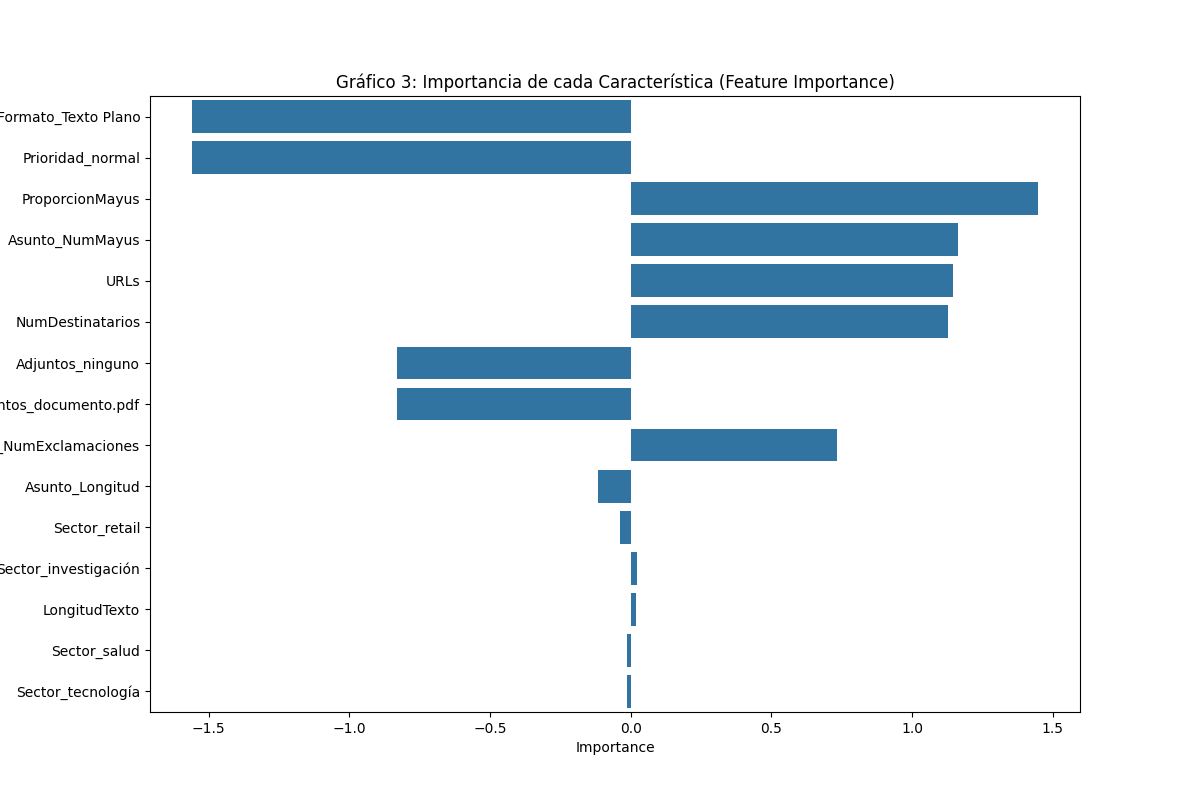
\includegraphics[width=0.9\textwidth]{grafico_3_importancia_features.png}

\subsection{Gráfico 4: Distribución de probabilidades y umbrales}
Este gráfico ilustra cómo el modelo asigna probabilidades a cada correo. Se incluye el umbral por defecto (0.5) y el umbral óptimo calculado con el índice J de Youden. La separación casi perfecta entre SPAM y HAM refuerza la sospecha de un dataset poco realista.

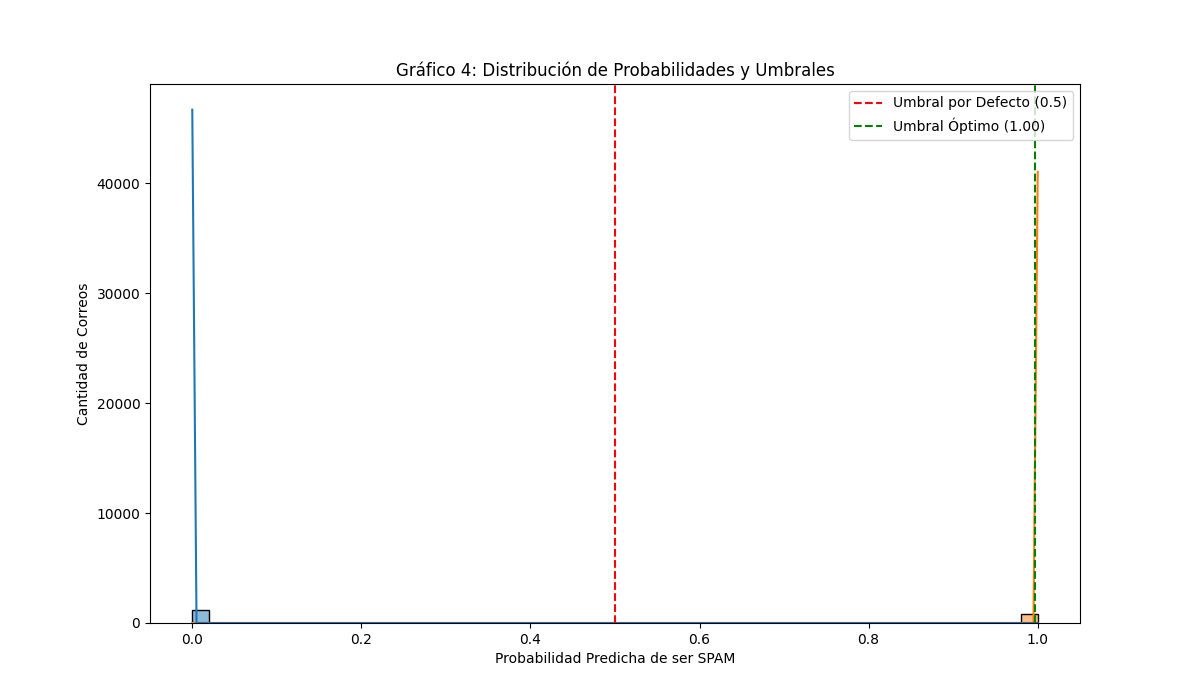
\includegraphics[width=0.9\textwidth]{grafico_4_distribucion_probabilidades.png}

\section{Discusión Crítica}
Un modelo que alcanza un 100\% de precisión genera preocupaciones importantes:

\begin{itemize}
    \item En la práctica, los datasets reales de correos contienen errores, mensajes ambiguos y características redundantes.
    \item Un desempeño perfecto sugiere \textbf{sobre ajuste} o la existencia de variables soplones que simplifican la clasificación.
    \item Al evaluar el modelo con validación cruzada, se observó que el F1-Score y la exactitud mantenían valores altos, reforzando la idea de un dataset artificial.
\end{itemize}

Esto significa que, aunque el modelo parece excelente en laboratorio, no se puede garantizar su desempeño en un entorno real, donde los atacantes adaptan sus técnicas constantemente.

\section{Conclusiones}
\begin{enumerate}
    \item La regresión logística es una técnica potente para problemas de clasificación binaria como SPAM vs HAM.
    \item La creación de nuevas variables derivadas del asunto y la fecha aporta valor explicativo.
    \item Un dataset demasiado perfecto puede conducir a interpretaciones erróneas del rendimiento del modelo.
    \item Es fundamental validar el modelo en escenarios más realistas y considerar métricas robustas como el F1-Score, que combina precisión y exhaustividad.
\end{enumerate}

\section*{Apéndice: Código}

\begin{lstlisting}
print("Script final iniciado. Generando todos los analisis para el informe...")
import pandas as pd
import numpy as np
import seaborn as sns
import matplotlib.pyplot as plt
from sklearn.model_selection import train_test_split, cross_val_score
from sklearn.preprocessing import StandardScaler
from sklearn.linear_model import LogisticRegression
from sklearn.metrics import confusion_matrix, classification_report, roc_curve, roc_auc_score

# --- CARGAR Y PREPARAR DATOS ---
try:
    df = pd.read_csv('email_dataset.csv')
except FileNotFoundError:
    print("Error: Asegurate de que tu archivo CSV ('email_dataset.csv') este en la misma carpeta.")
    exit()

# Mapeamos etiquetas
etiqueta_map = {'spam': 1, 'ham': 0}
df['Clase'] = df['Clase'].map(etiqueta_map)
df.dropna(subset=['Clase'], inplace=True)
df['Clase'] = df['Clase'].astype(int)

# Eliminamos soplones directos
df = df.drop(columns=['FrecuenciaPalabrasSpam', 'ErroresOrtograficos', 'Cuerpo'], errors='ignore')

# Creamos features
df['Asunto_Longitud'] = df['Asunto'].astype(str).apply(len)
df['Asunto_NumExclamaciones'] = df['Asunto'].astype(str).apply(lambda x: x.count('!'))
df['Asunto_NumMayus'] = df['Asunto'].astype(str).apply(lambda x: sum(1 for c in x if c.isupper()))

# Extraemos la hora de la fecha
df['Hora'] = pd.to_datetime(df['FechaHora']).dt.hour

# Definimos features finales
features_finales = [
    'LongitudTexto',
    'ProporcionMayus',
    'URLs',
    'NumDestinatarios',
    'Asunto_Longitud',
    'Asunto_NumExclamaciones',
    'Asunto_NumMayus',
    'Hora',
    'Formato',
    'Sector',
    'Prioridad',
    'Adjuntos'
]

# Reaplicamos encoding solo a las categoricas necesarias
df_encoded = pd.get_dummies(df[features_finales + ['Clase']], 
                            columns=['Formato', 'Sector', 'Prioridad', 'Adjuntos'], 
                            drop_first=True)

# --- ANALISIS DE CORRELACION ---
print("\nGenerando analisis de correlacion...")
numeric_features = [
    'LongitudTexto', 'ProporcionMayus', 'URLs', 
    'NumDestinatarios', 'Asunto_Longitud', 
    'Asunto_NumExclamaciones', 'Asunto_NumMayus', 'Hora'
]
correlation_matrix = df[numeric_features + ['Clase']].corr()

# Grafico 1: Matriz de Correlacion
plt.figure(figsize=(10, 8))
sns.heatmap(correlation_matrix, annot=True, cmap='coolwarm', fmt=".2f")
plt.title('Grafico 1: Matriz de Correlacion de Features Numericas')
plt.savefig('grafico_1_correlacion.png')
print("Grafico 1 guardado como 'grafico_1_correlacion.png'")

# --- SELECCION DE CARACTERISTICAS Y DIVISION DE DATOS ---
X = df_encoded.drop(columns=['Clase'])
y = df_encoded['Clase']

X_train, X_test, y_train, y_test = train_test_split(
    X, y, test_size=0.2, random_state=42, stratify=y
)

# --- CONSTRUCCION Y ENTRENAMIENTO DEL MODELO LOGISTICO ---
print("\nConstruyendo y entrenando el modelo de Regresion Logistica...")
scaler = StandardScaler()
X_train_scaled = scaler.fit_transform(X_train)
X_test_scaled = scaler.transform(X_test)

model = LogisticRegression(max_iter=10000)
model.fit(X_train_scaled, y_train)
print("Modelo entrenado")

# --- PREDICCIONES Y METRICAS DE ERROR ---
y_pred = model.predict(X_test_scaled)
y_pred_prob = model.predict_proba(X_test_scaled)[:, 1]

# Metricas de error y rendimiento
accuracy = (y_pred == y_test).mean()
error_rate = 1 - accuracy
report = classification_report(y_test, y_pred, output_dict=True)
precision_spam = report['1']['precision']
f1_spam = report['1']['f1-score']

print("\n--- Metricas de Rendimiento y Error ---")
print(f"Exactitud (Accuracy): {accuracy:.4f}")
print(f"Tasa de Error: {error_rate:.4f}")
print(f"Precision para SPAM: {precision_spam:.4f}")
print(f"F1-Score para SPAM: {f1_spam:.4f}")
print("---------------------------------------")

# --- ANALISIS DETALLADO Y GRAFICOS ---

# Grafico 2: Matriz de Confusion
cm = confusion_matrix(y_test, y_pred)
plt.figure(figsize=(8, 6))
title = f'Grafico 2: Matriz de Confusion (sobre {len(y_test)} muestras de prueba)'
sns.heatmap(cm, annot=True, fmt='d', cmap='Blues', xticklabels=['HAM', 'SPAM'], yticklabels=['HAM', 'SPAM'])
plt.xlabel('Prediccion del Modelo')
plt.ylabel('Valor Real')
plt.title(title)
plt.savefig('grafico_2_matriz_confusion.png')
print("Grafico 2 guardado como 'grafico_2_matriz_confusion.png'")

# Grafico 3: Importancia de Caracteristicas
importances = pd.DataFrame(data={'Feature': X.columns, 'Importance': model.coef_[0]})
importances = importances.sort_values(by='Importance', key=abs, ascending=False)
plt.figure(figsize=(12, 8))
sns.barplot(x='Importance', y='Feature', data=importances.head(15))
plt.title('Grafico 3: Importancia de cada Caracteristica (Feature Importance)')
plt.savefig('grafico_3_importancia_features.png')
print("Grafico 3 guardado como 'grafico_3_importancia_features.png'")

# Grafico 4: Distribucion de Probabilidades y Umbrales
fpr, tpr, thresholds_roc = roc_curve(y_test, y_pred_prob)
optimal_idx = np.argmax(tpr - fpr)
optimal_threshold = thresholds_roc[optimal_idx]

plt.figure(figsize=(12, 7))
sns.histplot(x=y_pred_prob, hue=y_test, kde=True, bins=50)
plt.title('Grafico 4: Distribucion de Probabilidades y Umbrales')
plt.xlabel('Probabilidad Predicha de ser SPAM')
plt.ylabel('Cantidad de Correos')
plt.axvline(0.5, color='red', linestyle='--', label=f'Umbral por Defecto (0.5)')
plt.axvline(optimal_threshold, color='green', linestyle='--', label=f'Umbral Optimo ({optimal_threshold:.2f})')
plt.legend()
plt.savefig('grafico_4_distribucion_probabilidades.png')
print("Grafico 4 guardado como 'grafico_4_distribucion_probabilidades.png'")

# --- VALIDACION CRUZADA ---
print("\nEjecutando validacion cruzada (5 folds)...")
scores_f1 = cross_val_score(model, scaler.transform(X), y, cv=5, scoring='f1')
scores_acc = cross_val_score(model, scaler.transform(X), y, cv=5, scoring='accuracy')

print("\n--- Validacion Cruzada ---")
print(f"F1 promedio: {scores_f1.mean():.4f} +/- {scores_f1.std():.4f}")
print(f"Accuracy promedio: {scores_acc.mean():.4f} +/- {scores_acc.std():.4f}")
print("--------------------------")

print("\nProceso completado! Revisa los 4 archivos .png y los resultados en consola.")
\end{lstlisting}

\end{document}
